\section{Descriptive Similarity}
There exists a kind of similarity among different articles, although the stories from the different articles are totally discrepant, they may have the same structure of the stories.
\\
\begin{figure}[!hbp]
\centering
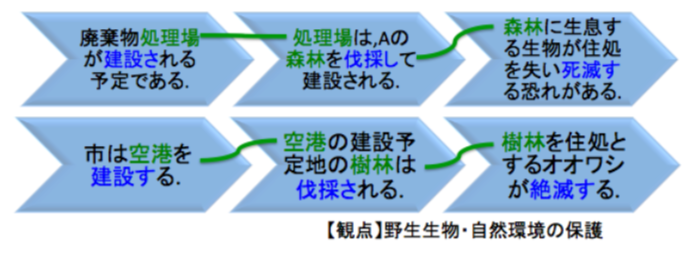
\includegraphics[width=350pt]{./pictures/0102.png}
\caption{descriptive similarity}
\end{figure}
\\
From the example giving in the figure, we can easily understand the descriptive similarity between different articles among the accept of text structure. [10]
\\
Among articles with the descriptive similarity, we can say,
\begin{enumerate}
\item The structure of equivalents is similar.
\item The article contains similar stories.
\end{enumerate}
We call this kind of similarity the descriptive similarity. We would like to extract it among different articles.
Here are two stories to makes is more easy to understand descriptive similarity between different stories.[13]\\ \\
Story 1 
\begin{CJK}{UTF8}{ipxm}
\textbf{あやしい牛}
\end{CJK}
\\ \\ 
\begin{CJK}{UTF8}{ipxm}
昔、福井は夜になっても大勢の人が行き交う、とても栄えた町だった。\\
ところがある夜から、金色の二つの光を持った化け物が現れ、町の八百屋を荒らして回るようになった。怖がった人々は夜に出歩かなくなり、町はだんだんとさびれていった。\\
困った若者たちが、夜の八百屋を見張っていると、化け物の正体はどうやら牛である事が分かった。すると牛飼いと名乗る不思議な老人が現れ、怪しい牛は「どこかの看板から抜け出た牛ではないか」と言う。そこで、町の薬屋の木彫りの牛の看板を確認すると、牛の蹄(ひづめ)にはまだ湿った土が付いていた。\\
彫り物の名人である「左甚五郎」作の立派な木彫りの牛が、夜な夜な看板から抜け出して福井の町を荒らしまわっていたのだった。牛飼いの老人が、看板の牛の両目と前足にノミで傷を入れると、二度と町中に怪しい牛が出没する事も無くなった。\\
それ以来、福井の町は再びにぎわいを取り戻した。その後しばらくして、八幡神社の境内に小さなお堂が建てられ、この牛の看板を大切に奉った。\\
\end{CJK}\\ \\
Story 2 
\begin{CJK}{UTF8}{ipxm}
\textbf{あばれ鹿}
\end{CJK}\\ \\
\begin{CJK}{UTF8}{ipxm}
昔、伊豆は函南村(かんなみむら)の辺りでは、夜な夜な2頭のつがいの大鹿が現れ、田畑を荒らしまわるので、村人は大層困っていた。そこで村人は、猟師の勘七(かんしち)に大鹿を退治してくれるよう頼んだ。\\
勘七は火縄銃を持つと、猟犬とともに狩野川(かのがわ)の川べりにやってきた。そこで夜が来るのを待ち、大鹿を待ち伏せようというのだ。\\
さて、夜になると、勘七が思ったとおり2頭の夫婦(めおと)の大鹿が手前の畑に現れた。勘七は、大鹿を火縄銃が撃てる所まで引き付けるため、猟犬を大鹿の後ろからけしかけた。猟犬にけしかけられた大鹿は、勘七の目論見どおり勘七の前に走って来る。\\
ところが、2頭の大鹿は勘七の目の前で大きく飛び跳ねたのだ。勘七は不意を突かれたものの、かろうじて雄鹿を撃つことが出来た。しかし、勘七の放った弾は確かに雄鹿に命中したのだが、不思議なことに雄鹿の姿はどこにも見当らなかった。\\
夜が明けてから勘七が辺りを見回すと、2頭の鹿の足跡が村の方へと続いている。勘七が足跡を追うと、それは興聖寺(こうしょうじ)の境内で途切れていた。勘七が住職に事情を話し、寺の本堂を調べていると、勘七の猟犬は住職の寝室の方に向かって吠えている。勘七が寝室を開けると、そこには見事な夫婦の鹿の襖絵(ふすまえ)があった。勘七が近づいて見てみれば、なんと雄鹿の胸には勘七に鉄砲で撃たれた傷があるではないか。\\
この大鹿の襖絵は、さる高名な絵師によって描かれたもので、その出来栄えがあまりに見事だったゆえ、ふすまの中から大鹿が現れ出たのだった。しかしこの夫婦の大鹿、勘七に鉄砲で撃たれてからは、恐れをなしたのか、襖の中から出て来ることは二度となかったそうだ。\\
\end{CJK}\\
These pair of stories come from different provinces in Japan. While they seem to be talking about the different things that happen in completely different palaces, but we can easily see that all the stories have a similar process: wired animals come out from some places, destroys the crop and affects the people's life. With the help of capable people, the animals return to their original place and the country isin harmony again.
So far we have introduced the definition of descriptive similarity and gave an example of it. Our research is to extract descriptive pattern base on descriptive similarity.